\documentclass[12pt, letterpaper]{article}
\usepackage[top=2.5cm, bottom=2.5cm, left=3cm, right=2.5cm]{geometry}
\usepackage[utf8]{inputenc}
\usepackage[T1]{fontenc}
\usepackage{lmodern}
\usepackage{amsmath, amssymb}
\usepackage{booktabs}
\usepackage{tabularx}
\usepackage{longtable}
\usepackage{array}
\usepackage{multirow}
\usepackage{xcolor}
\usepackage{graphicx}
\usepackage{float}
\usepackage{listings}
\usepackage[most, breakable]{tcolorbox}
\usepackage{enumitem}
\usepackage{fancyhdr}
\usepackage{titlesec}
\usepackage{setspace}
\usepackage{microtype}
\usepackage[hidelinks]{hyperref}
\usepackage{parskip}
\usepackage{tikz}
\usetikzlibrary{positioning}
\usepackage{pgfplots}
\pgfplotsset{compat=1.15}
\usepackage{tikz}
\usepackage{pgfplots}
% Colours
\definecolor{econblue}{RGB}{31,78,121}
\definecolor{researchgreen}{RGB}{21,101,45}
\definecolor{exampleorange}{RGB}{180,80,20}
\definecolor{lightgray}{RGB}{245,245,245}
\definecolor{boxblue}{RGB}{220,235,248}

% Section headings
\titleformat{\section}{\large\bfseries\color{econblue}}{\thesection}{1em}{}%
  [\vspace{-4pt}\rule{\linewidth}{0.4pt}]
\titleformat{\subsection}{\normalsize\bfseries\color{econblue}}{\thesubsection}{1em}{}
\titleformat{\subsubsection}{\normalsize\bfseries}{\thesubsubsection}{1em}{}

% Page style
\pagestyle{fancy}
\fancyhf{}
\fancyhead[L]{\small\itshape ECON 230 --- Introduction to Behavioural Economics}
\fancyhead[R]{\small\itshape Chapter 8: Irrational Markets}
\fancyfoot[C]{\small\thepage}
\renewcommand{\headrulewidth}{0.4pt}
\setlength{\headheight}{14pt}

% tcolorbox styles
\tcbuselibrary{breakable, skins, listings}

\newtcolorbox{researchbox}{
  enhanced, breakable,
  colback=researchgreen!6, colframe=researchgreen!55,
  title=\textbf{Research Study},
  fonttitle=\bfseries\small,
  attach boxed title to top left={yshift=-2mm, xshift=6mm},
  boxed title style={colback=researchgreen!55, colframe=researchgreen!55},
  before upper={\setlength{\parskip}{4pt}}
}

\newtcolorbox{examplebox}[1]{
  enhanced, breakable,
  colback=exampleorange!6, colframe=exampleorange!45,
  title=\textbf{#1}, fonttitle=\bfseries\small
}

\newtcolorbox{keybox}{
  enhanced, colback=boxblue, colframe=econblue!70,
  fontupper=\small
}

% ASCII figure style
\lstset{
  basicstyle=\scriptsize\ttfamily,
  breaklines=false,
  keepspaces=true,
  columns=flexible,
  frame=single,
  backgroundcolor=\color{lightgray},
  xleftmargin=4pt, xrightmargin=4pt,
  aboveskip=6pt, belowskip=6pt
}

% Lists
\setlist[itemize]{leftmargin=1.5em, itemsep=2pt, topsep=4pt}
\setlist[enumerate]{leftmargin=1.5em, itemsep=2pt, topsep=4pt}
\onehalfspacing

\newcolumntype{Y}{>{\raggedright\arraybackslash}X}

\begin{document}

\begin{titlepage}
\centering\vspace*{3cm}
{\Large\bfseries\color{econblue} ECON 230 --- Introduction to Behavioural Economics\\[1em]}
{\large\bfseries Course Textbook\\[2em]}
{\LARGE\bfseries\color{econblue} Chapter 8\\[0.5em]}
{\Large\bfseries Irrational Markets --- Behavioural Finance\\[2em]}
\vfill
{\normalsize University of Northern British Columbia\\
Instructor: Prof.\ Muhebullah Karimzada\\
Term: Winter 2027}
\end{titlepage}
\tableofcontents
\newpage


\medskip


\section*{Chapter Overview}
\addcontentsline{toc}{section}{Chapter Overview}


The previous seven chapters have documented cognitive biases, social preferences, and bounded rationality at the level of individual decision-making. This chapter asks a natural and important question: do these individual-level deviations from rationality aggregate into market-level mispricings? Or does financial market competition --- with its powerful incentives, rapid feedback, and ability to attract sophisticated participants --- correct individual biases before they affect prices?

The answer, developed over four decades of research, is nuanced. Markets are remarkably efficient in many respects --- most available information is rapidly incorporated into prices, and most professional investors consistently fail to beat the market after fees. But systematic, persistent, and economically significant anomalies coexist with this general efficiency. Asset prices are too volatile relative to changes in fundamental value. Individual stocks exhibit momentum that persists over months. Investors hold too much of their home country's stocks despite the large efficiency gains available from international diversification. And occasionally, financial markets produce spectacular bubbles and crashes that cannot be explained by any reasonable model of rational investors responding to changing fundamentals.

\textbf{Behavioural finance} is the field that explains these phenomena by applying the tools of behavioural economics --- prospect theory, overconfidence, heuristics, herding, and limits to arbitrage --- to financial markets. It does not claim that markets are useless or that prices are random. It claims that prices are sometimes wrong in predictable directions, and that understanding \textit{why} they are wrong requires understanding the psychology of the investors who set them.

This chapter proceeds from the benchmark of the \textbf{Efficient Market Hypothesis} (EMH) --- the claim that prices reflect all available information --- through the anomalies that challenge it, through the formal model of limits to arbitrage that explains why rational investors cannot always correct mispricings, and through a series of documented market phenomena that behavioural finance has illuminated: bubbles, the disposition effect, home bias, overconfident trading, and herding. We close with a behavioural post-mortem of the 2008 global financial crisis and the 2020--2022 Canadian housing boom and bust.

\medskip


\section*{Learning Objectives}
\addcontentsline{toc}{section}{Learning Objectives}


After studying this chapter, students should be able to:

\begin{enumerate}
\item \textbf{Define} the Efficient Market Hypothesis in its three forms and evaluate the evidence for each.
\item \textbf{Explain} the noise trader model (De Long et al., 1990) and identify the key result that noise traders can earn higher expected returns than rational arbitrageurs.
\item \textbf{State} the three sources of limits to arbitrage (Shleifer and Vishny, 1997) and explain why they prevent rational investors from correcting mispricings.
\item \textbf{Describe} the anatomy of an asset price bubble and identify the behavioural mechanisms that drive the expansion and collapse phases.
\item \textbf{Explain} the disposition effect in financial markets, cite the evidence from Odean (1998), and identify its economic costs and contribution to momentum.
\item \textbf{Define} home bias, quantify its magnitude for Canadian investors, and explain it using familiarity, availability, and overconfidence.
\item \textbf{Describe} the overconfidence trading evidence (Barber and Odean, 2001) and explain the mechanism linking overconfidence to excess trading and lower returns.
\item \textbf{Explain} herding and informational cascades and describe how they can produce correlated errors across sophisticated institutional investors.
\item \textbf{Identify} the major market anomalies (momentum, value premium, excess volatility) and assess whether they represent genuine market inefficiency or rational risk premia.
\item \textbf{Conduct a behavioural post-mortem} of the 2008 global financial crisis, identifying the specific biases that contributed at each stage, and evaluate Canada's relative resilience.
\end{enumerate}

\medskip


\section*{Introduction: When Rational Investors Create Irrational Markets}
\addcontentsline{toc}{section}{Introduction: When Rational Investors Create Irrational Markets}


In March 2000, Cisco Systems --- the dominant manufacturer of internet networking equipment --- reached a market capitalisation of \$555 billion. At that moment, Cisco was the most valuable company in the world. To determine whether this valuation was justified, financial analysts ran a straightforward discounted cash flow calculation.

The result was uncomfortable. To generate sufficient future earnings to justify a \$555 billion valuation at any reasonable discount rate, Cisco would need to:
\begin{itemize}
\item Grow at approximately \textbf{80\% per year for ten consecutive years}, and then
\item Sustain growth at \textbf{20\% per year} indefinitely thereafter.
\end{itemize}

The first requirement would make Cisco larger than the entire US economy by year ten. The second is physically impossible for a finite economy. The Cisco valuation was, by any fundamental calculation, deeply impossible to justify.

Did the investors who paid these prices know this? Almost certainly, yes. Many of them were sophisticated professionals with access to the same discounted cash flow models. Did they invest anyway? The data shows they did. Cisco's stock had risen 500\% in the preceding five years. The NASDAQ composite index --- dominated by technology stocks --- rose 527\% between 1995 and its peak in March 2000. Then it fell 77\%, reaching its trough in October 2002. Amazon shares fell from a peak of \$107 to \$5.97. Pets.com raised \$82 million in an IPO, reached a market capitalisation of \$290 million, and was delisted nine months later with a share price of \$0.19.

The dot-com bubble is not an exception in financial history. It is a recurring pattern. Tulip bulbs in seventeenth-century Holland. South Sea Company shares in 1720 England. Railway stocks in 1840s Britain. Japanese real estate and equities in the 1980s. US housing in 2003--2006. Canadian housing in 2020--2022. Bitcoin and other cryptocurrencies in multiple cycles. The pattern recurs too consistently across centuries and asset classes to be dismissed as coincidence or idiosyncrasy.

\textbf{Behavioural finance} is the project of understanding why. Not why markets are simply inefficient, but why sophisticated investors --- armed with information, with incentives to get prices right, and with the full arsenal of modern financial analysis --- repeatedly and collectively price assets at levels that fundamental analysis cannot justify, and then watch as prices collapse.

\medskip


\section{The Efficient Market Hypothesis}



\subsection{The Benchmark}


The \textbf{Efficient Market Hypothesis} (EMH), developed primarily by Eugene Fama in a landmark 1970 paper, is the central benchmark of finance theory. Its core claim: \textbf{asset prices at any moment fully reflect all available information}. This means no trading strategy based on available information can consistently earn risk-adjusted returns above the market average.

The intuition is competitive: if a price were too low given available information, investors would buy it, driving the price up until the profit opportunity disappeared. If a price were too high, investors would sell it short, driving it down. Competition among informed, rational investors ensures that price deviations from fundamental value are rapidly corrected.

Fama identified three forms of the EMH, differing in what "available information" means:

\textbf{Weak Form:} Past prices and trading volumes contain no information that can generate abnormal returns. Price changes are unpredictable from historical prices. Technical analysis --- the practice of looking for patterns in price charts --- adds no value.

\textbf{Semi-Strong Form:} All publicly available information --- past prices, earnings announcements, dividend declarations, economic data, analyst reports --- is already incorporated in prices. Fundamental analysis based on public information adds no value.

\textbf{Strong Form:} All information, including private (insider) information, is reflected in prices. Even insiders cannot consistently earn abnormal returns. This is the most extreme form and is widely regarded as empirically false --- the existence of securities law prohibiting insider trading would be unnecessary if this were true.


\subsection{Evidence in Favour of Market Efficiency}


The case for market efficiency is substantial:

\textbf{Active managers persistently underperform.} The most powerful evidence for EMH comes from the performance of professional fund managers. If active management --- selecting stocks on the basis of research, analysis, and judgment --- consistently added value, we would expect professional managers to consistently beat the market. The evidence shows the opposite.

The S\&P Indices Versus Active (SPIVA) Canada Scorecard tracks the performance of Canadian actively managed mutual funds against their benchmark indices. In 2023, over a 15-year horizon:
\begin{itemize}
\item \textbf{91\%} of Canadian active equity funds underperformed their benchmark indices, net of fees.
\item The average underperformance was approximately 1.5 percentage points per year.
\item Funds that outperformed in one five-year period showed little tendency to outperform in the next.
\end{itemize}

This near-universal underperformance over long horizons is consistent with the semi-strong form of EMH: if prices already reflect all publicly available information, active managers who use that information cannot expect to systematically beat the market.

\textbf{Sharpe's arithmetic.} Nobel laureate William Sharpe (1991) provided a simple but profound argument for why this must be so. The average investor must earn the market return before fees --- by definition, since all investors collectively \textit{are} the market. After fees, the average active investor must therefore earn \textit{below} the market return. Since passive investors (who hold the index) pay lower fees, the average passive investor must earn more than the average active investor. Beating the market through active management is not impossible, but it is necessarily a zero-sum game in which any winner's gains come at the expense of another active investor's losses --- before fees.

\textbf{Random walks and price unpredictability.} Extensive statistical testing of stock price sequences has found that past prices have very limited predictive power for future prices, consistent with the weak form. Price changes behave approximately as a random walk, with autocorrelations close to zero at most horizons.


\subsection{Evidence Against Market Efficiency: Anomalies}


Despite the powerful case for EMH, a systematic body of evidence documents \textbf{market anomalies} --- patterns in returns that are inconsistent with simple versions of the hypothesis. The most robust anomalies include:

\textbf{Excess volatility.} Robert Shiller (1981) --- who would share the Nobel Prize in Economics in 2013 with Eugene Fama, in one of the more ironic joint awards in Nobel history --- showed that stock prices are far more volatile than can be justified by changes in future dividends. If prices reflect the present value of future dividends (the fundamental value), and if dividends are relatively smooth, then prices should be relatively smooth too. In fact, prices fluctuate far more widely than dividends, suggesting that a substantial component of price variation is unrelated to fundamental value.

\textbf{Momentum.} Jegadeesh and Titman (1993) documented that stocks that performed well over the past 3--12 months continue to outperform stocks that performed poorly over the same period --- for the subsequent 3--12 months. This \textbf{momentum anomaly} generates risk-adjusted abnormal returns that have been replicated across many countries, time periods, and asset classes (including commodities, currencies, and bonds). It is inconsistent with the weak form of EMH if it represents a genuine inefficiency.

\textbf{Value premium.} Fama and French (1992, 1993) documented that "value stocks" --- stocks with low price-to-book ratios, low price-to-earnings ratios, or high dividend yields --- have historically earned higher returns than "growth stocks" with the opposite characteristics. This value premium is one of the most replicated findings in empirical finance.

\textbf{Post-earnings-announcement drift.} When a company announces earnings that substantially exceed or miss analyst expectations, the share price moves in the direction of the surprise --- but then continues to drift in the same direction for months afterward. This \textbf{underreaction} to earnings news is inconsistent with the semi-strong EMH if the information is publicly available.

\textbf{Table 8.1: Major Market Anomalies and Their Potential Explanations}


\begin{table}[H]
\centering
\small
\begin{tabularx}{\linewidth}{lYYY}
\toprule
Anomaly & Finding & Efficient Market Explanation & Behavioural Explanation \\
\midrule
Excess volatility & Prices are too volatile vs dividends (Shiller 1981) & Discount rate variation & Investor sentiment, animal spirits \\
Momentum & Past winners continue to win (3--12 months) & Priced risk factor & Underreaction, disposition effect, herding \\
Value premium & Low P/B stocks earn higher returns & Compensation for distress risk & Overextrapolation, representativeness heuristic \\
Post-earnings drift & Prices drift in direction of earnings surprise & Statistical artefact & Underreaction to public information \\
Closed-end fund puzzle & Closed-end funds trade at discounts to NAV & Transaction costs, taxes & Investor sentiment, limits to arbitrage \\
Home bias & Investors over-invest in domestic stocks & Legal, information advantages & Familiarity, availability, overconfidence \\
Disposition effect & Investors sell winners, hold losers & Tax-loss harvesting (losers), tax realisation (winners) & Loss aversion, reference-dependence \\
\bottomrule
\end{tabularx}
\end{table}


The existence and persistence of these anomalies is the central empirical challenge to the EMH and the primary motivation for behavioural finance.

\medskip


\section{Limits to Arbitrage}



\subsection{Why Smart Money Doesn't Fix Prices}


The standard defence of EMH against anomalies runs as follows: even if irrational investors create mispricings, rational arbitrageurs --- large, sophisticated investors who identify the mispricing --- will trade against it, profiting as they drive prices back to fundamental value. The rational investors make money; the irrational investors lose money and eventually exit the market. In the long run, prices converge to fundamentals.

This is a powerful argument, and it is sometimes correct. But Shleifer and Vishny (1997) identified three structural reasons why arbitrage is risky and limited in practice --- reasons why rational investors cannot always correct mispricings before they become large and persistent.


\subsection{Source 1: Fundamental Risk}


\textbf{Arbitrage is never truly risk-free.} In the textbook definition, arbitrage is the simultaneous purchase and sale of identical assets at different prices, generating certain profit with no capital at risk. In practice, this pure arbitrage rarely exists in financial markets. More commonly, the "arbitrage" trade involves:
\begin{itemize}
\item \textbf{Buying the underpriced asset} (say, a technology stock that appears cheap based on fundamentals), financed by
\item \textbf{Selling short a similar but not identical asset} (say, another technology stock as a hedge).
\end{itemize}

If the assets are not perfectly identical, the trade carries \textbf{fundamental risk}: the two assets may move differently, so the trade can lose money even if the mispricing never closes. No perfect substitute for an individual company's shares exists --- you cannot hedge your long position in Nortel by shorting a perfectly correlated asset, because no such asset exists.


\subsection{Source 2: Noise Trader Risk}


Even if fundamental risk is manageable, a rational investor who takes a position against a mispricing faces a further problem: the mispricing may get \textbf{worse before it gets better}.

Suppose a rational investor identifies that Company X is overvalued by 30\% and short-sells its shares. A group of irrationally optimistic noise traders then drives the price up another 30\%. The rational investor is now sitting on a loss --- they have been correct about the fundamental analysis, but they are losing money because the irrational investors are, in the short run, moving prices further from fundamental value.

This creates \textbf{noise trader risk}: the risk that an arbitrageur who is correct about fundamentals will lose money in the short run because irrational sentiment pushes prices in the wrong direction before correcting. Crucially, this risk is not diversifiable --- it is a systematic feature of the arbitrage trade, present in every bet against mispricing.

The 1997 paper by De Long, Shleifer, Summers, and Waldmann (actually from 1990, a foundational paper) formalises this. Their model shows:

\begin{itemize}
\item In a world with both rational arbitrageurs and noise traders (investors who trade on sentiment), noise traders can \textbf{earn higher expected returns} than rational arbitrageurs --- because they bear more risk (noise trader risk).
\item Noise traders who happen to be optimistic about the market tend to hold riskier portfolios; the risk premium on those portfolios compensates them for the risk, on average.
\item Because rational arbitrageurs fear short-run amplification of mispricing, they trade only partially against it, leaving some mispricing uncorrected at equilibrium.
\item Prices can deviate substantially and persistently from fundamental values even in a world where some investors are fully rational.
\end{itemize}

The famous phrase --- "Markets can remain irrational longer than you can remain solvent" --- attributed to Keynes, captures this mechanism precisely. A rational investor who correctly identifies an overvaluation can go broke waiting for prices to correct.


\subsection{Source 3: Agency Costs and Short Investment Horizons}


The third limit to arbitrage is institutional. Most sophisticated investors do not manage their own money --- they manage funds on behalf of clients (pension funds, endowments, high-net-worth individuals). This creates \textbf{principal-agent problems} between fund managers (agents) and their investors (principals).

The critical feature: fund managers are typically evaluated over short horizons (quarterly, annually) relative to benchmarks. A manager who correctly identifies a mispricing may underperform their benchmark for months or years before the mispricing corrects. During this period, investors may withdraw capital from the fund, the manager may lose their job, or the fund may be liquidated.

Shleifer and Vishny (1997) called this the "limits to arbitrage" problem: \textbf{arbitrageurs with short time horizons and career concerns behave myopically}, reducing their positions in losing trades even when those trades are fundamentally correct. The rational response to this institutional environment is to avoid the very trades that would move prices toward fundamental value.

This mechanism helps explain the persistence of bubbles: sophisticated investors may recognise a bubble but avoid betting against it because the career costs of being early --- underperforming peers for an extended period before the collapse --- outweigh the expected gains. As Keynes noted in a different context: "It is better to fail conventionally than to succeed unconventionally."

\begin{researchbox}
\textbf{Research Study: The Limits of Arbitrage --- Siamese Twin Companies}\\[4pt]

\textbf{Researchers:} Kenneth Froot and Emil Dabora\\[4pt]
\textbf{Year:} 1999\\[4pt]
\textbf{Research Question:} Can rational arbitrage prevent persistent mispricings in securities where the fundamental value relationship is unambiguous?\\[4pt]
\textbf{Background:} Royal Dutch Shell and Shell Transport and Trading Company were separate companies that agreed in 1907 to merge their interests in a fixed 60:40 ratio --- meaning Royal Dutch should always be worth exactly 1.5 times the market value of Shell Transport, since both represent claims on the same underlying cash flows.\\[4pt]
\textbf{Results:} Despite this fixed fundamental relationship, the relative prices of the two shares deviated significantly and persistently from the 60:40 parity. Royal Dutch was sometimes underpriced by up to 35\% relative to its fundamental value; at other times Shell Transport was underpriced. These deviations persisted for years before correcting.\\[4pt]
\textbf{Economic Interpretation:} The deviation from parity represented an apparently risk-free arbitrage opportunity --- buy the cheap share, sell the expensive one in the fixed ratio. Yet sophisticated hedge funds that attempted this trade (including Long-Term Capital Management) suffered large losses because the mispricing continued to widen before correcting. The trade was correct in fundamental terms but ruinous in practice due to noise trader risk and short investment horizons.\\[4pt]
\textbf{Behavioural Insight:} Even in a case where the correct fundamental relationship is unambiguously defined by contract, mispricings can persist because the institutional and risk environment makes arbitrage costly and dangerous. This "near-arbitrage" failure is one of the most compelling direct demonstrations that limits to arbitrage are real and consequential.\\[4pt]
\end{researchbox}

\newpage


\section{The Noise Trader Model}



\subsection{The Two-Type Framework}


The De Long, Shleifer, Summers, and Waldmann (1990) model --- the DSSW model --- provides the most important theoretical framework in behavioural finance. It establishes the conditions under which irrational investors can not only survive but thrive in financial markets, and explains why rational arbitrage cannot fully correct mispricings.

The model features two types of investors:

\textbf{Rational arbitrageurs (sophisticated investors):} These investors know the fundamental value of all assets and have rational expectations about future prices. They maximise expected utility, taking account of all available information and all sources of risk.

\textbf{Noise traders:} These investors trade on pseudosignals --- beliefs about asset values that are uncorrelated with fundamental value. They might follow technical analysis, react to market sentiment, extrapolate past trends, or simply follow the crowd. Their beliefs about prices are systematically distorted by psychological biases.

Both types of investors invest in a risky asset (whose fundamental value is known to rational arbitrageurs) and a safe asset.


\subsection{The Surprising Conclusion}


The DSSW model demonstrates a counterintuitive result: \textbf{noise traders can earn higher average returns than rational arbitrageurs} despite (or rather because of) their systematic misvaluation of assets.

The mechanism: noise traders tend to be more optimistic about the risky asset (on average) than its fundamental value warrants. They therefore hold more of the risky asset. Because they hold more of the risky asset, they are exposed to more risk --- including the risk that their own sentiment shifts unfavourably. This extra risk generates a risk premium: noise traders earn higher average returns as compensation for bearing more risk.

Rational arbitrageurs, meanwhile, recognise the existence of noise trader risk --- the risk that sentiment will move against them in the short run --- and therefore hold less of the risky asset than they would without noise traders. Their portfolio is conservative, earning lower average returns.

\textbf{The policy implication} is troubling: noise traders are not automatically selected against by market competition. They earn competitive or superior returns despite their irrationality, which means they are not driven out of the market. Financial markets can sustain a persistent population of noise traders even in a world where sophisticated rational investors coexist.


\subsection{Sentiment and Asset Prices}


Building on the DSSW framework, Baker and Wurgler (2006, 2007) developed an empirical measure of \textbf{investor sentiment} --- the overall optimism or pessimism of retail investors about the stock market --- and showed that it has significant predictive power for future stock returns.

In periods of high sentiment, retail investors are optimistic and bid up the prices of "sentiment-sensitive" stocks --- small stocks, young companies, high-volatility stocks, and stocks with no earnings history. In subsequent periods, these stocks tend to underperform as sentiment reverts toward its mean. The direction of predictability is negative: high sentiment today predicts low returns tomorrow, consistent with overvaluation driven by optimistic noise traders.

This finding is difficult to reconcile with the EMH but fits naturally with the noise trader model: sentiment shifts represent distortions to prices that rational arbitrageurs cannot fully correct due to the limits studied in Section 2.

\medskip


\section{Asset Price Bubbles}



\subsection{What Is a Bubble?}


An \textbf{asset price bubble} is a sustained and significant overvaluation of an asset relative to its fundamental value, driven by investor expectations of continued price appreciation rather than by the intrinsic return the asset will generate. Bubbles end in crashes: sharp and rapid corrections toward (or below) fundamental value, typically accompanied by widespread investor losses and often by broader economic damage.

Defining a bubble precisely is challenging. We can only assess whether an asset was overvalued \textit{ex ante} if we can independently estimate its fundamental value --- which is difficult for assets with uncertain future cash flows. Nevertheless, some historical episodes are so extreme that the bubble characterisation is uncontroversial: the Cisco example from the introduction is one such case.

\textbf{Figure 8.1: A Timeline of Major Historical Bubbles}
\begin{figure}[h!]
\centering

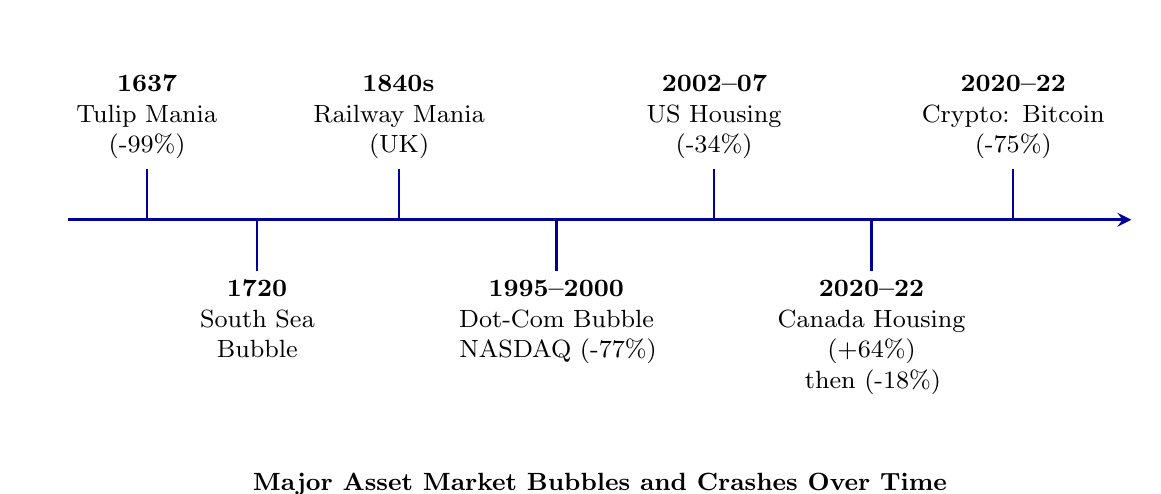
\begin{tikzpicture}[
    >=stealth,
    timeline/.style={very thick, blue!60!black},
    event/.style={thick, blue!60!black},
    label/.style={
        font=\small,
        align=center,
        text width=2.8cm
    }
]

% Timeline
\draw[timeline,->] (0,0) -- (13.5,0);

% ---- Above timeline ----

% 1637 Tulip Mania
\draw[event] (1,0) -- (1,0.65);
\node[label, above=0.65cm of {(1,0)}] 
{\textbf{1637}\\Tulip Mania\\(-99\%)};

% 1840s Railway Mania
\draw[event] (4.2,0) -- (4.2,0.65);
\node[label, above=0.65cm of {(4.2,0)}]
{\textbf{1840s}\\Railway Mania\\(UK)};

% 2002-07 Housing
\draw[event] (8.2,0) -- (8.2,0.65);
\node[label, above=0.65cm of {(8.2,0)}]
{\textbf{2002--07}\\US Housing\\(-34\%)};

% 2020-22 Crypto
\draw[event] (12,0) -- (12,0.65);
\node[label, above=0.65cm of {(12,0)}]
{\textbf{2020--22}\\Crypto: Bitcoin\\(-75\%)};


% ---- Below timeline ----

% South Sea Bubble
\draw[event] (2.4,0) -- (2.4,-0.65);
\node[label, below=0.65cm of {(2.4,0)}]
{\textbf{1720}\\South Sea\\Bubble};

% Dot-Com
\draw[event] (6.2,0) -- (6.2,-0.65);
\node[label, below=0.65cm of {(6.2,0)}]
{\textbf{1995--2000}\\Dot-Com Bubble\\NASDAQ (-77\%)};

% Canada Housing
\draw[event] (10.2,0) -- (10.2,-0.65);
\node[label, below=0.65cm of {(10.2,0)}]
{\textbf{2020--22}\\Canada Housing\\(+64\%) then (-18\%)};


% Axis label
\node[below=1.9cm,font=\small]
at (6.75,-1.2)
{\textbf{Major Asset Market Bubbles and Crashes Over Time}};

\end{tikzpicture}

\caption{Historical examples of asset price bubbles and subsequent corrections.}
\label{fig:bubbles_timeline}

\end{figure}

\begin{table}[H]
\centering
\small
\begin{tabularx}{\linewidth}{lYYYY}
\toprule
Period & Asset & Peak Overvaluation & Crash Magnitude & Behavioural Drivers \\
\midrule
1637 & Dutch Tulip Bulbs & Extraordinary & ~99\% & Social proof, scarcity narrative, extrapolation \\
1720 & South Sea Company & ~10$\times$ fundamental & ~84\% & Narrative ("trade monopoly"), momentum \\
1840s & UK Railways & Large & ~85\% & Technology narrative, extrapolation \\
1925--29 & US Stocks & ~3$\times$ fair value & ~89\% & Leverage, momentum, narrative \\
1985--89 & Japan (stocks + real estate) & ~4$\times$ fundamental & ~62\% (stocks) & Low rates, keiretsu cross-holdings \\
1995--2000 & US Technology (NASDAQ) & Large & ~77\% & Technology narrative, overconfidence, availability \\
2003--06 & US Housing & ~50\% overvalued & ~34\% national & Low rates, leverage, complexity, originate-to-distribute \\
2020--22 & Canadian Housing & +64\% in 2 years & ~18\% & Low rates, FOMO, extrapolation \\
2017--21 & Cryptocurrencies & Multiple cycles & ~75--85\% & Novelty narrative, FOMO, retail herding \\
\bottomrule
\end{tabularx}
\end{table}



\subsection{The Anatomy of a Bubble}


Asset price bubbles follow a recognisable pattern, described by economist Hyman Minsky (1986) and later popularised by Charles Kindleberger (1978, 2000) in the classic work \textit{Manias, Panics, and Crashes}. The Minsky-Kindleberger framework identifies five stages:

\textbf{Stage 1: Displacement.} A new technology, low interest rates, a policy change, or an external shock creates a genuine improvement in some assets' prospects. Early investors profit. The narrative of a "new era" begins to develop. (Examples: the internet in 1993; Bank of Canada rates cut to 0.25\% in March 2020.)

\textbf{Stage 2: Boom.} Rising prices attract more investors. Credit availability expands. New investors enter the market, many with limited experience of previous cycles. Extrapolation of recent price gains becomes the dominant forecasting method. The narrative becomes mainstream. Prices begin to disconnect from fundamentals.

\textbf{Stage 3: Euphoria.} Valuation concerns are dismissed or rationalised. "This time is different" arguments proliferate. Leverage increases. New, less-sophisticated investors enter at the top. Warning voices are ridiculed as missing the new paradigm. Rational arbitrageurs who have bet against the bubble have already suffered losses.

\textbf{Stage 4: Financial Distress.} Some early investors --- and eventually insiders --- begin to sell. Prices plateau. A triggering event reveals that some of the speculative investments are fundamentally unsound. Credit tightens. Leveraged investors face margin calls. The narrative shifts.

\textbf{Stage 5: Revulsion.} Prices collapse rapidly as forced selling accelerates. Leverage amplifies the decline. Investors who were "buying the dip" absorb losses. The narrative reverses completely --- the asset is now seen as worthless. Prices may overshoot below fundamental value.

\textbf{Behavioural mechanisms driving each stage:}

\begin{itemize}
\item \textbf{Extrapolation and representativeness:} Past price gains are treated as representative of future returns (Chapter 2). "Tech stocks always go up" becomes a heuristic.
\item \textbf{Availability:} Recent dramatic examples of gains are highly available in memory, inflating perceptions of likely return (Chapter 2).
\item \textbf{Overconfidence:} Investors overestimate their ability to identify the right assets and the right exit timing (Chapter 2).
\item \textbf{FOMO (Fear of Missing Out):} Seeing others profit creates social proof and peer pressure. Not investing is coded as a loss relative to a social reference point (Chapter 3).
\item \textbf{Narrative economics:} Compelling stories about why this time is different substitute for rigorous fundamental analysis (Shiller, 2019).
\item \textbf{Herding:} Investors follow the crowd, partly rationally (inferring information from others' actions) and partly due to social conformity (Chapter 6).
\end{itemize}


\subsection{The Dot-Com Bubble}


The dot-com bubble of 1995--2000 is the most thoroughly studied financial bubble of the modern era and provides the clearest demonstration of the DSSW framework and its limits.

The NASDAQ composite index rose from approximately 750 in January 1995 to approximately 5,048 at its peak in March 2000 --- a gain of 574\%. It then fell to approximately 1,140 in October 2002 --- a decline of 77\% from the peak. The round trip took seven years.

\textbf{The fundamental disconnect.} At the peak, companies like Cisco, Amazon, and hundreds of smaller dotcoms were valued at multiples of revenue --- not earnings, which were typically negative --- that implied growth rates physically impossible to sustain. The standard discounted cash flow analysis, applied correctly, produced valuations far below prevailing market prices for almost all major technology stocks.

Why did prices reach these levels? Several behavioural mechanisms were simultaneously operative:

\textbf{Extrapolation of past returns.} The tech sector had genuinely produced extraordinary returns in the preceding five years. Investors who extrapolated these returns into the future were using the representativeness heuristic --- past performance was seen as representative of future performance --- even though the theoretical justification for such expectations was absent.

\textbf{The technology narrative.} The internet was a genuine technological revolution that created enormous value. The fact that it would create enormous value was used to justify any price. The logical gap --- between "the internet will be important" and "therefore this specific unprofitable company at this specific price is fairly valued" --- was overlooked in the enthusiasm.

\textbf{Availability and social proof.} Stories of overnight fortunes created by early internet investments were extremely available. Social proof --- everyone around you is investing and getting rich --- provided a powerful heuristic endorsement for the strategy.

\textbf{Overconfidence.} Individual investors who had made money in the rising market attributed their success to skill rather than to the general market appreciation. This overconfidence led them to concentrate positions and take on leverage.

\textbf{The role of institutional investors.} Perhaps most surprisingly, institutional investors --- pension funds, endowments, and professional fund managers --- participated enthusiastically in the bubble, despite having access to fundamental analysis. The limits to arbitrage partly explain this: a fund manager who avoided tech stocks in 1998--1999 dramatically underperformed peers, faced redemptions, and risked losing their mandate. The career incentives pushed professional investors toward the bubble rather than away from it.


\subsection{The 2020--2022 Canadian Housing Boom}


The Canadian housing market experienced its most dramatic price appreciation in modern history between 2020 and early 2022, followed by a significant correction. The episode illustrates how the same behavioural mechanisms that drive financial market bubbles also operate in less liquid real asset markets.

\textbf{The displacement:} In March 2020, the Bank of Canada cut its overnight lending rate from 1.75\% to 0.25\% in response to the COVID-19 pandemic --- the lowest rate in Canadian history. Fixed and variable mortgage rates fell correspondingly. At these rates, the same monthly mortgage payment could finance a substantially larger home purchase.

\textbf{The boom:} Canadian average home prices rose 64\% between early 2020 and their peak in February 2022. In some markets --- Greater Toronto, Vancouver, and secondary cities like Hamilton and Kitchener --- price increases were even more dramatic. Multiple-offer scenarios became standard, with purchasers bidding 20--30\% above asking prices without conditions (no financing condition, no inspection condition).

\textbf{The behavioural mechanisms:}
\begin{itemize}
\item \textbf{FOMO (Fear of Missing Out):} In a market with rapidly rising prices and well-publicised stories of buyers priced out of the market, waiting to purchase felt increasingly costly. The social comparison reference point (Chapter 3) was the peer who had bought the previous year; being priced out relative to that peer registered as a loss.
\item \textbf{Availability and extrapolation:} Canadian house prices had risen in most markets for over 20 years. The scenario of a sharp national price decline was essentially absent from recent experience --- and therefore cognitively unavailable (Chapter 2). Most buyers expected modest continued appreciation at minimum.
\item \textbf{Social proof and narrative:} Media coverage was saturated with housing price stories. Stories of 30\% bidding premiums and 10-offer situations were widely available, reinforcing the sense that not buying was the riskiest strategy.
\item \textbf{Loss aversion at the margin:} In the framing of purchasing decisions, "being priced out forever" was coded as a large prospective loss, while "overpaying by 10\%" was a smaller certain loss. Prospect theory predicts that in the loss domain, people are risk-seeking --- they take the gamble (pay above asking without conditions) to avoid the certain loss of being priced out.
\end{itemize}

\textbf{The crash:} The Bank of Canada raised interest rates from 0.25\% to 5.0\% between March 2022 and July 2023 --- the most rapid rate increase in Canadian history. Average national home prices fell approximately 18\% from their February 2022 peak. In some markets, the decline exceeded 25\%.

The behavioural finance of the decline was equally interesting:
\begin{itemize}
\item \textbf{Nominal loss aversion and price stickiness (Chapter 3):} Sellers who had purchased near the 2022 peak refused to list at prices below their purchase price. The Genesove-Mayer (2001) mechanism operated at scale: loss-averse sellers withdrew listings rather than accept nominal losses, reducing transaction volumes.
\item \textbf{Variable-rate mortgage shock:} Approximately 300,000 Canadian households with variable-rate mortgages experienced payment shocks as rates rose. The psychological impact of a sharp increase in obligatory monthly outflows --- framed as a loss relative to the prior payment reference point --- was substantially more aversive than the prospect theory model predicts a pure income effect would generate.
\end{itemize}

\medskip


\section{The Disposition Effect in Financial Markets}



\subsection{The Pattern and Its Cost}


The \textbf{disposition effect} was introduced in Chapter 3 as a prediction of Prospect Theory: because the value function is concave in the gain domain and convex in the loss domain, investors should prefer to sell winning positions (locking in a certain gain in the concave region) and hold losing positions (gambling on recovery in the convex region).

The real-world evidence for the disposition effect in actual market behaviour is among the most robust findings in empirical finance.

Odean (1998) analysed the complete trading records of 10,000 individual brokerage accounts over the period 1987--1993. The key measure: the \textbf{Proportion of Gains Realised (PGR)} relative to the \textbf{Proportion of Losses Realised (PLR)}. If investors treated gains and losses symmetrically, PGR and PLR should be equal. The data showed:

\begin{itemize}
\item \textbf{PGR = 14.8\%:} In any given period, investors sold 14.8\% of their "paper gain" positions.
\item \textbf{PLR = 9.8\%:} They sold only 9.8\% of their "paper loss" positions.
\item Investors were \textbf{52\% more likely} to realise a gain than an equivalent loss.
\end{itemize}

This was not a rational tax strategy. If anything, rational tax planning predicts the \textit{opposite}: investors should sell losses to realise tax deductions and defer gains to defer tax liabilities. The actual pattern is the reverse of what tax optimisation would require.

The economic cost is large. Odean computed the subsequent performance of the stocks that were sold (winners) and the stocks that were held (losers):
\begin{itemize}
\item \textbf{Stocks sold (winners):} Earned an average of \textbf{+3.4\%} in the year after the sale.
\item \textbf{Stocks held (losers):} Earned an average of \textbf{-1.1\%} in the year after they were not sold.
\end{itemize}

The round-trip cost of the disposition effect --- selling good stocks and holding bad ones --- was approximately \textbf{4.4 percentage points} of annual return. Compounded over decades, this is an enormous drag on wealth accumulation.

\textbf{Figure 8.2: The Disposition Effect --- Proportions Realised}

\begin{figure}[ht]
\centering

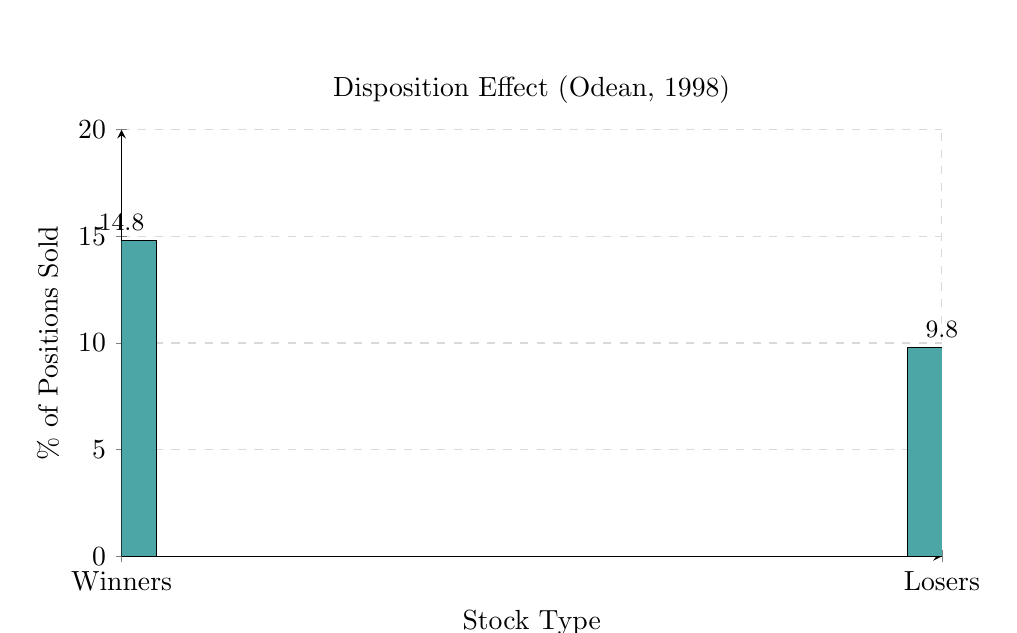
\begin{tikzpicture}
\begin{axis}[
    ybar,
    bar width=25pt,
    width=12cm,
    height=7cm,
    ymin=0,
    ymax=20,
    ylabel={\% of Positions Sold},
    xlabel={Stock Type},
    xtick={1,2},
    xticklabels={Winners,Losers},
    enlarge x limits=0.5,
    axis lines=left,
    grid=major,
    grid style={dashed,gray!30},
    nodes near coords,
    nodes near coords style={
        font=\small,
        anchor=south
    },
    title={Disposition Effect (Odean, 1998)},
    legend style={
        at={(0.5,-0.18)},
        anchor=north,
        legend columns=2
    }
]

% Both bars in one plot
\addplot[
    fill=teal!70,
    draw=black
] coordinates {
    (1,14.8)
    (2,9.8)
};



\end{axis}
\end{tikzpicture}

\caption{Disposition effect: investors are more likely to sell winning stocks than losing stocks.}
\label{fig:disposition_effect}

\end{figure}


\begin{table}[H]
\centering
\small
\begin{tabularx}{\linewidth}{lY}
\toprule
 & Description \\
\midrule
\textbf{What the figure shows} & A bar chart with two bars: PGR (Proportion of Gains Realised = 14.8\%) shown in teal and PLR (Proportion of Losses Realised = 9.8\%) shown in red. The teal bar is notably taller than the red bar. \\
\textbf{How to interpret it} & The 52\% difference in the likelihood of selling a winner versus an equivalent loser is the disposition effect. Both bars should be equal if investors treated gains and losses symmetrically. The gap is attributable to the asymmetric risk attitudes predicted by Prospect Theory: risk aversion in the gain domain produces the tendency to lock in gains, while risk seeking in the loss domain produces the tendency to gamble on recovery. \\
\bottomrule
\end{tabularx}
\end{table}



\subsection{The Disposition Effect and Momentum}


The disposition effect has an important market-level consequence: it contributes to the \textbf{momentum anomaly} documented in Section 1.3.

The mechanism: when a stock rises, many investors are sitting on paper gains. The disposition effect makes them sellers --- they realise gains and exit the position. This selling pressure partially offsets the price rise, causing the stock to \textbf{underreact} to good news initially. Subsequently, as the good news gradually registers and selling pressure abates, the stock continues to rise --- producing the momentum pattern of continued appreciation following good performance.

Conversely, when a stock falls, loss-averse investors hold their positions rather than selling. This reduces the supply of shares for sale, limiting the price decline and causing \textbf{underreaction} to bad news. Subsequently, as the bad news is gradually incorporated, the stock continues to fall --- producing the momentum pattern of continued depreciation following bad performance.

This behavioural model of momentum --- proposed by Grinblatt and Han (2005) --- provides a coherent explanation for one of the most robust anomalies in finance, rooted directly in the Prospect Theory mechanisms of Chapters 3.

\medskip


\section{Home Bias}



\subsection{The Puzzle}


\textbf{Home bias} refers to the tendency of investors to hold a disproportionately large share of their portfolios in domestic assets, relative to what international diversification would prescribe. It is one of the most well-documented puzzles in international finance.

The optimal portfolio under modern portfolio theory (Markowitz, 1952; Tobin, 1958) is the global market portfolio: investors should hold each country's assets in proportion to their share of total world market capitalisation. Canada represents approximately \textbf{3\% of world equity market capitalisation}. An optimally diversified Canadian investor should hold approximately 3\% of their equity portfolio in Canadian stocks and 97\% in international stocks.

The actual holdings of Canadian investors bear little resemblance to this prescription. French and Poterba (1991), in the founding study of home bias, found that investors in every country held dramatically more domestic equities than the optimum suggests. Updated figures for Canadian investors:

\textbf{Table 8.2: Home Bias in Canadian Equity Portfolios}


\begin{table}[H]
\centering
\small
\begin{tabularx}{\linewidth}{lYY}
\toprule
 & Canadian Stocks & International Stocks \\
\midrule
\textbf{Canada's share of world market cap} & ~3\% & ~97\% \\
\textbf{Typical Canadian retail investor portfolio} & ~50\% & ~50\% \\
\textbf{Optimal portfolio (CAPM)} & ~3\% & ~97\% \\
\textbf{Over-concentration ratio} & ~17$\times$ & n/a \\
\bottomrule
\end{tabularx}
\end{table}


The over-concentration in Canadian stocks --- holding 17 times the optimal international allocation in domestic equities --- represents an enormous forfeit of diversification benefits. A portfolio concentrated in Canadian stocks is highly exposed to commodity price risk (Canada's economy is resource-intensive), housing market risk (bank stocks represent a large share of the TSX), and country-specific macro risks that an internationally diversified portfolio would diversify away.


\subsection{Why Home Bias Persists}


Standard economics offers some rational explanations for home bias: information advantages (domestic investors know more about local companies), currency risk (domestic assets are denominated in the investor's home currency), transaction costs, and legal restrictions on international investment. These explanations have some validity --- but they cannot explain the magnitude of the home bias, particularly in an era of low-cost international index funds, exchange-traded funds, and global information flow.

The behavioural explanations are more powerful:

\textbf{Familiarity heuristic.} Huberman (2001) documented that investors systematically prefer to invest in companies they are familiar with --- their own utility company, their bank, companies headquartered in their city. This familiarity is mistaken for safety: familiar companies feel less risky, even when objective measures of risk (volatility, correlation with the investor's income) are identical. Canadian investors know what the Royal Bank does; they are less familiar with Deutsche Bank, despite both being large, diversified commercial banks with similar risk profiles.

\textbf{Availability.} Canadian stocks are more cognitively available to Canadian investors than international stocks: they appear in local news, are discussed in Canadian financial media, and form the basis of most discussions of investment in the Canadian context. More available stocks are judged to be better and safer investments, consistent with the availability heuristic (Chapter 2).

\textbf{Overconfidence about local knowledge.} Canadian investors may overestimate the value of their local information advantage relative to the expertise of global fund managers who analyse international markets full-time (Chapter 2). This overconfidence in home market knowledge justifies concentrating in the home market.

\textbf{Loss aversion and reference points.} For Canadian investors, Canadian stocks define the reference point for portfolio performance. Underperforming Canadian stocks (a loss relative to reference) is more psychologically aversive than underperforming a global index (which is less salient as a reference point). This makes concentration in Canadian stocks feel "safer" even when it is objectively riskier.


\subsection{The Economic Cost}


The economic cost of home bias is substantial. A Canadian investor who held 50\% Canadian stocks and 50\% international stocks over the period 1990--2020 would have significantly underperformed an investor who held the global market cap weights --- both because the Canadian market underperformed global markets in that period (due to its commodity-heavy composition) and because the diversification benefits of international holdings were not fully captured.

Beyond returns, the risk cost is also significant. Canadian stocks are highly correlated with each other (they move together with commodity prices, housing market conditions, and Canadian economic cycles). International diversification reduces portfolio volatility substantially --- a benefit that concentrated domestic portfolios forgo.

\medskip


\section{Overconfidence and Excess Trading}



\subsection{The Mechanism}


Chapter 2 documented overconfidence as a pervasive feature of human judgment. In financial markets, overconfidence takes a specific form: investors overestimate the value and accuracy of their private information about stock prices. They believe they know something the market does not --- that a specific stock is undervalued, that a market trend will continue, that a particular investment strategy will outperform.

This overconfidence leads to \textbf{excess trading}: investors buy and sell more frequently than is optimal, because they believe each trade reflects a genuine information advantage rather than noise. Rational investors who understood that their private information is no better than the market's would simply hold the index. Overconfident investors trade frequently, generating transaction costs and tax liabilities that drag on returns.

Odean (1999) formalised this prediction: overconfident investors will trade too much, and the costs of excess trading (commissions, bid-ask spreads, market impact, taxes) will outweigh the benefits (the exploitation of genuine information advantages that turn out, on average, to be illusory).


\subsection{The Evidence}


\begin{researchbox}
\textbf{Research Study: Boys Will Be Boys --- Gender, Overconfidence, and Investment Returns}\\[4pt]

\textbf{Researchers:} Brad Barber and Terrance Odean\\[4pt]
\textbf{Year:} 2001\\[4pt]
\textbf{Research Question:} Does overconfidence lead investors to trade excessively, and does excess trading destroy returns?\\[4pt]
\textbf{Method:} Barber and Odean analysed a dataset of 35,000 household brokerage accounts from a major US discount broker, covering the period 1991--1997. They used the psychology literature's finding that men exhibit significantly higher overconfidence than women (particularly in financial domains) to predict that men would trade more than women. They then compared trading frequency and net investment returns between male and female account holders.\\[4pt]
\textbf{Results}\\[4pt]
- Men's annual portfolio turnover: \textbf{77\%} (they replaced 77\% of their portfolio, on average, each year)
- Women's annual portfolio turnover: \textbf{53\%}
- Men's net annual return relative to buy-and-hold: \textbf{-1.4 percentage points}
- Women's net annual return relative to buy-and-hold: \textbf{-0.94 percentage points}
- The gap attributable to excess trading: approximately \textbf{0.46 percentage points per year}

Single men traded even more and underperformed by approximately 1.9 percentage points annually relative to single women.

\textbf{Economic Interpretation:} The pattern is exactly what overconfidence predicts: investors who trade more (overconfident investors, predominantly men) earn lower net returns, because their trades reflect noise rather than information. The transaction costs of excess trading --- commissions, bid-ask spreads, taxes on realised gains --- are not offset by any systematic informational advantage.\\[4pt]

\textbf{Behavioural Insight:} The Barber and Odean finding does not imply that women are better investors in some fundamental sense. It implies that lower overconfidence --- less trading --- is more consistent with rational investment behaviour in markets where most private "information" is noise. The optimal response to financial markets, for most investors, is to trade rarely and hold the index.\\[4pt]
\end{researchbox}


\newpage

\textbf{Figure 8.3: Trading Frequency and Returns by Gender}

\begin{figure}[ht]
\centering

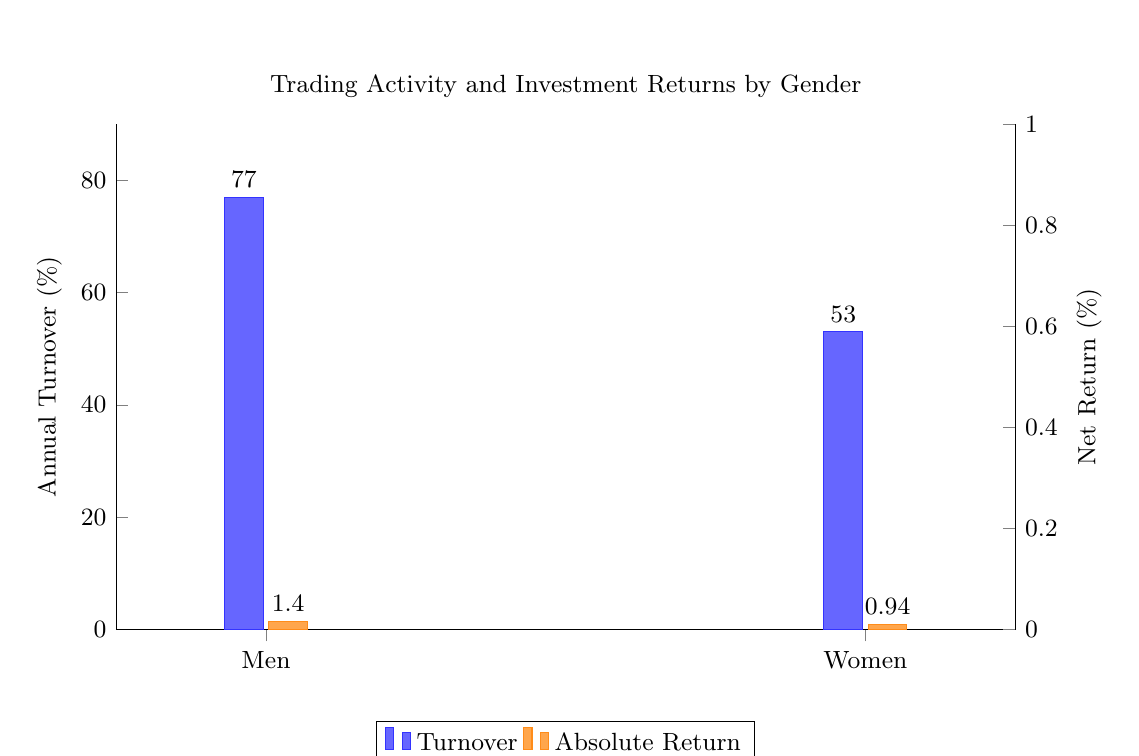
\begin{tikzpicture}

\begin{axis}[
    width=13cm,
    height=8cm,
    ybar,
    bar width=14pt,
    enlarge x limits=0.25,
    symbolic x coords={Men,Women},
    xtick=data,
    ylabel={Annual Turnover (\%)},
    ymin=0,
    ymax=90,
    axis y line*=left,
    axis x line*=bottom,
    nodes near coords,
    nodes near coords style={
        font=\small,
        anchor=south
    },
    title={\small Trading Activity and Investment Returns by Gender},
    legend style={
        at={(0.5,-0.18)},
        anchor=north,
        legend columns=2,
        font=\small
    },
    tick label style={font=\small},
    ylabel style={font=\small},
]


% Turnover bars
\addplot[
    fill=blue!60,
    draw=blue!80
]
coordinates {
    (Men,77)
    (Women,53)
};

\addlegendentry{Turnover}


% Returns on same axis but scaled
\addplot[
    fill=orange!70,
    draw=orange!90
]
coordinates {
    (Men,1.4)
    (Women,0.94)
};

\addlegendentry{Absolute Return}


\end{axis}


% Right axis for returns
\begin{axis}[
    width=13cm,
    height=8cm,
    symbolic x coords={Men,Women},
    xtick=\empty,
    axis y line*=right,
    axis x line=none,
    ylabel={Net Return (\%)},
    ymin=0,
    ymax=2,
    tick label style={font=\small},
    ylabel style={font=\small},
    legend style={draw=none}
]

\end{axis}

\end{tikzpicture}

\caption{Trading behaviour and investment performance by gender. Men exhibit higher portfolio turnover, while both groups experience negative net returns.}
\label{fig:gender_trading}

\end{figure}


\begin{table}[H]
\centering
\small
\begin{tabularx}{\linewidth}{lY}
\toprule
 & Description \\
\midrule
\textbf{What the figure shows} & A paired bar chart with four bars. The first pair shows annual portfolio turnover: men's turnover (77\%) as a blue bar and women's turnover (53\%) as a shorter blue bar. The second pair shows net annual returns relative to buy-and-hold: men's return (-1.4\%) as a short red bar below the zero line and women's return (-0.94\%) as a slightly smaller red bar also below zero. \\
\textbf{How to interpret it} & Both groups underperform a buy-and-hold strategy, confirming that trading generally destroys returns. Men underperform by more because they trade more. The higher their trading activity (reflecting overconfidence), the greater the underperformance. The figure is not about gender per se --- it is about overconfidence and its consequences. \\
\bottomrule
\end{tabularx}
\end{table}



\subsection{Implications for Retail Investors}


The Barber and Odean findings, combined with the SPIVA data on active fund managers, point to a clear prescription for retail investors: \textbf{passive, low-cost, diversified investing consistently outperforms most active strategies}, for both individual investors and professional fund managers, over long horizons.

This recommendation --- sometimes called the "passive investing" or "index investing" prescription --- is the most direct implication of behavioural finance for individual financial decision-making. It is not derived from a belief that markets are perfectly efficient, but from the recognition that:
\begin{enumerate}
\item The fees and transaction costs of active trading are large and certain.
\item The information advantages that would justify those costs are small and uncertain.
\item Overconfidence leads investors to overestimate their information advantage and therefore to trade more than is optimal.
\item The disposition effect, recency bias, and other psychological patterns systematically lead active investors to make suboptimal trade decisions.
\end{enumerate}

The rational response to recognising one's own cognitive limitations is not to eliminate trading (which is impossible) but to commit in advance to a rule-based, low-cost strategy that minimises the opportunities for psychological biases to cause harm.

\medskip


\section{Herding and Informational Cascades}



\subsection{Rational Herding}


Chapter 2 documented availability cascades --- the self-reinforcing cycles through which media coverage amplifies perceived risk beyond its actual level. In financial markets, a related mechanism produces \textbf{herding}: the tendency of investors to follow the actions of others, independently of their own private information.

Remarkably, herding can be \textbf{rational} --- not just a cognitive failure. The logic of \textbf{informational cascades} (Bikhchandani, Hirshleifer, and Welch, 1992) shows that it can be individually optimal to ignore one's private information and follow the crowd, even when the crowd is collectively wrong.

\textbf{The mechanism.} Suppose investors make investment decisions sequentially. Each investor has some private signal about the true value of an asset. The first investor acts on their signal. The second investor observes the first investor's action (but not their private signal) and incorporates this information into their decision. If the second investor's private signal agrees with the first's action, they follow it. If it disagrees, they might still follow the first --- because the first investor's action conveys information (they acted as if their signal was positive), which competes with the second investor's own (negative) signal.

By the time the fifth or tenth investor makes their decision, the accumulated information in prior investors' actions may be so large relative to any individual's private signal that it is rational for that investor to simply follow the crowd --- even if their private signal contradicts it. A cascade has formed: subsequent investors rationally ignore their private information, and the crowd converges on a single action regardless of the distribution of private signals.

\textbf{The vulnerability of cascades.} Information cascades can be based on very thin evidence --- the early movers' private signals. If those signals were wrong or the early movers made mistakes, the entire cascade can lead a large population of rational agents to the wrong conclusion. And because later movers have suppressed their private information, the cascade is fragile: a single public signal that contradicts it can unwind the entire herd immediately, generating the sharp reversals characteristic of financial markets.


\subsection{Irrational Herding and Institutional Pressures}


In financial markets, herding also arises from irrational sources and institutional pressures:

\textbf{Reputation concerns.} A fund manager who holds an unusual position and is wrong looks foolish; a fund manager who holds a consensus position and is wrong is in good company. Career incentives therefore push professional investors toward consensus positions, amplifying herding (Scharfstein and Stein, 1990).

\textbf{Window dressing.} Institutional investors often adjust their portfolios at quarter-end to show holdings in stocks that have performed well (and eliminate embarrassing losers) before reporting to clients. This practice amplifies momentum: popular winning stocks attract further buying at quarter-end, and unpopular losing stocks face selling pressure.

\textbf{Benchmark tracking.} Fund managers evaluated against an index benchmark have an incentive to hold stocks that closely resemble the benchmark composition. Significant deviations from the benchmark create "tracking error" that generates performance that diverges from the benchmark --- in either direction. Career-risk-averse managers minimise tracking error, creating a form of herding around the index composition.


\subsection{Correlated Errors and Systemic Risk}


The most economically dangerous form of herding is not individual investors following each other but \textbf{institutional investors making correlated errors} --- adopting similar models, similar assumptions, and similar risk exposures simultaneously.

This is the mechanism at the heart of the 2008 financial crisis. As the next section discusses, the largest and most sophisticated financial institutions in the world simultaneously:
\begin{itemize}
\item Used similar quantitative models to evaluate mortgage-backed securities.
\item Made similar assumptions about default correlations and house price appreciation.
\item Held similar exposures to the same underlying risk factors.
\end{itemize}

When those assumptions proved wrong, the correlated nature of the errors meant that all institutions suffered simultaneously --- producing the systemic crisis rather than the idiosyncratic failures that an uncorrelated error distribution would have generated.

\medskip


\section{A Behavioural Post-Mortem: The 2008 Global Financial Crisis}



\subsection{The Standard Narrative and Its Limits}


The 2008 global financial crisis is frequently explained through the lens of incentive misalignment: the "originate-to-distribute" model of mortgage lending, in which mortgage originators sold loans to securitisers who bundled them into mortgage-backed securities (MBS) and collateralised debt obligations (CDOs), separated the lender from the credit risk. Originators had no incentive to ensure loan quality since they didn't hold the loans; securitisers had no incentive since they sold the securities; ratings agencies had no incentive since they were paid by issuers; and investors had too little information to assess the true risks.

This narrative --- agency failures all the way down --- is correct as far as it goes. But it is incomplete. The crisis also involved a cascade of cognitive failures among the most sophisticated financial actors in the world. These actors were not fooled by opaque incentives; they made systematic errors that behavioural economics can identify and explain.


\subsection{The Behavioural Anatomy of the Crisis}


\textbf{Overconfidence in models.} The quantitative models used to price MBS and CDOs --- particularly the Gaussian copula model developed by David Li --- required assumptions about the correlation between mortgage defaults. Historical default correlations, estimated from the available data (roughly 1990--2005), were low. Modellers and investors were systematically overconfident in the model's accuracy and in the quality of the underlying data, which did not include a sample of a nationwide US house price decline.

\textbf{Availability and the absence of a prior crash.} The scenario of a nationwide US house price decline had not occurred in the post-WWII era. Because it was absent from recent experience --- and therefore cognitively unavailable --- most models treated it as having probability approximately zero. This is a dramatic manifestation of the availability heuristic (Chapter 2): the risk that cannot be recalled from memory is assigned negligible probability.

\textbf{Herding among institutions.} The major financial institutions --- Citigroup, Bear Stearns, Lehman Brothers, Merrill Lynch, Morgan Stanley, UBS, Deutsche Bank --- held strikingly similar exposures to MBS and CDO products. This correlated positioning meant that when the market for these products failed, all institutions suffered simultaneously --- creating the systemic crisis rather than isolated firm failures.

\textbf{Confirmation bias in ratings.} Rating agencies --- Moody's, S\&P, Fitch --- assigned AAA ratings to tranches of CDOs that subsequently suffered complete loss. Post-crisis investigations found that internal analysts who expressed concerns were overruled; that models were adjusted to produce desired ratings; and that the agencies systematically sought evidence confirming their ratings rather than evidence that might falsify them. This is the precise pattern of confirmation bias described in Chapter 2.

\textbf{Complexity and cognitive overload.} CDO-squared instruments --- CDOs of CDOs --- were genuinely difficult to analyse even with powerful computing resources and financial expertise. The complexity itself became a form of cognitive overload: investors who could not fully evaluate the instruments relied on ratings (overconfidence in rating agency accuracy) and herd behaviour (other sophisticated investors were buying, so it must be fine).

\textbf{Narrative Economics.} Shiller (2019) argues that the housing bubble was sustained by a compelling narrative: American home ownership was a core cultural value, house prices had never declined nationally in modern memory, the financial innovation of securitisation allowed risk to be distributed broadly and efficiently. These narratives reduced the cognitive burden of questioning the bubble's sustainability.

\textbf{Table 8.3: Behavioural Mechanisms in the 2008 Financial Crisis}


\begin{table}[H]
\centering
\small
\begin{tabularx}{\linewidth}{lYY}
\toprule
Mechanism & How It Operated & Chapter Reference \\
\midrule
Overconfidence & Overestimation of model accuracy; underestimation of tail risk & Ch. 2 \\
Availability bias & Absence of nationwide house price decline from historical experience $\rightarrow$ near-zero probability assigned & Ch. 2 \\
Herding & Correlated MBS/CDO exposures across all major institutions & Ch. 8 \\
Confirmation bias & Rating agency models tuned to produce desired AAA ratings & Ch. 2 \\
Cognitive overload & CDO-squared complexity prevented genuine risk assessment & Ch. 1 \\
Extrapolation & Historical house price appreciation extrapolated into default models & Ch. 2, 8 \\
Agency problems & Originate-to-distribute misaligned incentives & Ch. 6 (social preferences) \\
Limits to arbitrage & Short-sellers of MBS faced margin calls before crisis; Paulson exception & Ch. 8 \\
\bottomrule
\end{tabularx}
\end{table}



\subsection{Canada's Relative Resilience}


Canada experienced a much milder version of the 2008--09 recession than the United States, despite deep integration of the two economies. Canadian unemployment peaked at 8.7\% vs the US peak of 10\%; Canadian home prices fell modestly vs the US 34\% decline; no Canadian bank required a government bailout.

The reasons are partly institutional:
\begin{itemize}
\item Canadian mortgage regulations require CMHC (Canada Mortgage and Housing Corporation) insurance on all high-ratio mortgages (less than 20\% down payment). This insurance requirement incentivises strict underwriting standards.
\item Canadian banks operate under a conservative regulatory regime (OSFI --- Office of the Superintendent of Financial Institutions) that maintained higher capital requirements than US equivalents.
\item Canada had no equivalent subprime mortgage market: non-bank mortgage origination (the source of most US subprime lending) was far less developed.
\item Canadian banks were not heavily exposed to US MBS products --- their business models were more conservative.
\end{itemize}

But Canada's resilience also reflects partly better decision-making environments: institutions that removed the originate-to-distribute incentive misalignment and maintained skin-in-the-game requirements for mortgage lenders. Behavioural finance suggests that well-designed institutions can mitigate the impact of cognitive biases by structuring incentives to reduce the scope for motivated reasoning, herding, and overconfidence.

\medskip


\section{Market Anomalies: Irrational or Rational Risk Premia?}


A central controversy in finance is whether the anomalies documented above --- momentum, value premium, disposition effect, home bias --- represent genuine market inefficiency (prices wrong in ways that smart investors could exploit) or rational risk compensation (higher average returns earned in exchange for higher risk, which rational investors demand as compensation).


\subsection{The Risk-Based Alternative}


Eugene Fama and Kenneth French argued that the value premium --- the tendency of low P/B stocks to earn higher returns --- is compensation for a priced risk factor. Stocks of distressed companies (which tend to have low P/B ratios) perform especially poorly in bad economic times. Investors who hold value stocks are implicitly accepting worse performance exactly when they least want it (in recessions). A risk premium for this exposure is rational.

Similarly, momentum strategies perform poorly in specific circumstances (sharp market reversals following crashes), and this downside risk may justify the historical momentum premium as rational compensation.


\subsection{The Behavioural Alternative}


The behavioural interpretation --- that anomalies reflect cognitive errors --- makes different predictions about how they should respond to certain conditions. For example:

\begin{itemize}
\item If the momentum anomaly reflects the disposition effect and underreaction, it should be stronger among stocks with high proportions of individual investor ownership (since institutional investors have fewer cognitive biases).
\item If home bias reflects familiarity rather than rational information advantages, it should decrease as information costs fall (which it has, gradually, over the past three decades as global information access has improved).
\item If the value premium reflects overextrapolation of past growth (investors overpay for "glamour" stocks with high growth histories and underpay for "value" stocks), then the premium should be largest in market segments where overextrapolation is most prevalent.
\end{itemize}

Both risk-based and behavioural interpretations have found empirical support, and the truth is almost certainly a mixture of both. Some portion of observed return premia reflects rational risk compensation; some reflects cognitive error. Disentangling the two is one of the central challenges of empirical finance.

\medskip


\section*{Critical Thinking Questions}
\addcontentsline{toc}{section}{Critical Thinking Questions}



\subsection{Conceptual Questions}


\begin{enumerate}
\item The Efficient Market Hypothesis says that prices reflect all available information. If this is true, what information do the anomalies documented in this chapter (momentum, value premium, post-earnings drift) reveal? Are these anomalies consistent with a sophisticated version of the EMH that accounts for rational risk premia?
\end{enumerate}

\begin{enumerate}
\item The noise trader model shows that noise traders can earn higher average returns than rational arbitrageurs. Does this mean it is irrational to be a rational investor? What does this result imply about the survival of irrationality in competitive markets?
\end{enumerate}

\begin{enumerate}
\item Shleifer and Vishny identify three limits to arbitrage: fundamental risk, noise trader risk, and agency costs. Which of these do you find most compelling as an explanation for why rational investors cannot fully correct mispricings? Are there other limits you would add to the list?
\end{enumerate}

\begin{enumerate}
\item Asset price bubbles are described as "irrational." But individual investors who bought NASDAQ stocks in 1998 and sold in 1999 made large profits --- they were rational to participate given their beliefs and exit strategies. At what level (individual or collective) is a bubble irrational? Can a bubble consist entirely of individually rational decisions?
\end{enumerate}

\begin{enumerate}
\item The disposition effect is described as costly --- investors lose approximately 4\% per year by selling winners and holding losers. But some investors who held losers experienced recoveries, and some who sold winners missed further gains. How would you design a study to definitively establish that the disposition effect destroys value, rather than reflecting a rational strategy that sometimes fails?
\end{enumerate}

\begin{enumerate}
\item Home bias is described as irrational because it foregoes international diversification benefits. But a Canadian investor whose income, pension, and real estate are all exposed to Canadian economic conditions might rationally prefer domestic stocks as a partial inflation hedge. How much of observed home bias can be explained by rational hedging motives? What evidence would distinguish rational hedging from familiarity bias?
\end{enumerate}

\begin{enumerate}
\item The 2008 financial crisis involved both incentive misalignment (originate-to-distribute) and cognitive biases (overconfidence, availability, herding). Are these independent explanations for the crisis, or does incentive misalignment cause cognitive bias? Would better-aligned incentives have eliminated the cognitive failures as well?
\end{enumerate}

\begin{enumerate}
\item Momentum is the tendency of recent past winners to continue winning. The behavioural explanation links momentum to the disposition effect (underreaction due to selling winners). But momentum also exists in commodity prices, currencies, and fixed income markets --- asset classes not easily connected to the disposition effect. Does this suggest multiple mechanisms, or a unified explanation?
\end{enumerate}

\begin{enumerate}
\item Post-crisis, many financial institutions adopted more sophisticated risk models (CVA, stressed VaR) and held more capital. Does this institutional reform address the behavioural sources of the crisis (overconfidence, herding, availability bias), or does it only address the incentive and capital structure problems?
\end{enumerate}

\begin{enumerate}
\item The recommendation to passive investors is to buy a low-cost index fund and hold it through market fluctuations. But the research documents that most investors fail to do this --- they sell after market declines (availability-driven fear) and chase returns in rising markets. Is the passive investing prescription achievable for typical investors without structural support (automatic contributions, locked accounts)?
\end{enumerate}


\subsection{Application Questions}


\begin{enumerate}
\item You manage a \$500 million Canadian pension fund. Your investment committee has observed that your portfolio is 48\% in Canadian equities (compared to Canada's 3\% of world market cap). Using the home bias analysis, calculate the approximate diversification cost of this allocation. What would you recommend, and what institutional and behavioural barriers would you face in implementing a change?
\end{enumerate}

\begin{enumerate}
\item A technology company announces earnings that are 40\% above analyst expectations. Its stock price rises 8\% on the announcement day. Using the post-earnings-announcement drift anomaly, predict what you would expect to happen to the stock price over the next 3--6 months. Is this prediction consistent with the semi-strong form of the EMH?
\end{enumerate}

\begin{enumerate}
\item A large pension fund manager is considering whether to short-sell a technology company that appears significantly overvalued (trading at 150$\times$ earnings in a sector that historically trades at 25$\times$). Using Shleifer and Vishny's limits to arbitrage framework, identify the specific risks the manager faces and explain why a rational manager might decline to execute the trade even if certain the stock is overvalued.
\end{enumerate}

\begin{enumerate}
\item The Royal Bank of Canada has introduced a new digital investment platform and wants to use behavioural finance principles to improve retail investor outcomes. Design five specific features of the platform --- drawing directly on the evidence in this chapter --- that would help investors avoid the disposition effect, home bias, overconfidence-driven excess trading, and recency-driven return chasing.
\end{enumerate}

\begin{enumerate}
\item A startup mortgage lending company is designing its business model. Its venture capital backers want to implement an originate-to-distribute model (selling all mortgages to investors) to maximise loan origination volume. Using the 2008 crisis post-mortem, explain the behavioural and incentive risks of this model. Propose an alternative structure that would maintain origination volume while better managing the cognitive and incentive failures the crisis revealed.
\end{enumerate}

\begin{enumerate}
\item Canadian housing prices fell approximately 18\% from peak to trough in 2022--2023. Using the behavioural finance framework, explain why many economists were surprised by both the magnitude of the rise (64\%) and the limited extent of the subsequent decline. What specific biases affected the forecasts of economists, buyers, and sellers?
\end{enumerate}

\begin{enumerate}
\item A portfolio manager notices that her team consistently sells stocks after they have risen 20\% (locking in gains) and holds stocks that have fallen 20\% for at least six months (hoping for recovery). Using the disposition effect evidence, calculate the approximate annual cost to the fund if the team manages \$2 billion. Design a systematic portfolio review process that would reduce the disposition effect.
\end{enumerate}

\begin{enumerate}
\item You are a regulator designing rules for a new cryptocurrency exchange operating in Canada. Using the behavioural finance framework, identify four specific regulatory design features that would reduce the harm from cognitive biases (overconfidence, herding, availability, FOMO) on retail cryptocurrency investors. For each feature, explain the specific bias it targets and the mechanism through which it works.
\end{enumerate}

\begin{enumerate}
\item A financial advisor is meeting a client who has held a technology stock that has fallen 65\% from its purchase price. The client says: "I can't sell now --- I'd be locking in a huge loss. I'll wait for it to come back." Using prospect theory and the disposition effect evidence, explain what cognitive error the client is making and how you would frame the decision to help them see past it.
\end{enumerate}

\begin{enumerate}
\item In the wake of the 2021--2022 Canadian housing boom, many first-time buyers purchased homes at prices near the peak without conditions. Using loss aversion, FOMO, availability, and extrapolation as your analytical tools, write a brief post-mortem of the decision-making errors that led buyers to the peak. What would a well-designed "cooling-off period" policy for real estate need to include to be effective?
\end{enumerate}


\subsection{Discussion Questions}


\begin{enumerate}
\item Eugene Fama won the 2013 Nobel Prize for developing the Efficient Market Hypothesis; Robert Shiller won the same prize for documenting market inefficiencies. How can two contradictory positions win the same prize? Is the apparent contradiction resolvable --- is there a version of EMH consistent with the anomalies Shiller documented?
\end{enumerate}

\begin{enumerate}
\item The noise trader model predicts that irrational investors can survive and even thrive in competitive markets. This contrasts with the evolutionary argument that competition should eliminate irrationality. Under what conditions does competition eliminate irrationality, and under what conditions does it not? What determines whether financial markets fall into the first or the second category?
\end{enumerate}

\begin{enumerate}
\item Behavioural finance recommends passive, low-cost investing for retail investors. But if all investors followed this advice, prices would no longer reflect fundamental information --- because nobody would be doing fundamental analysis. Is the passive investing prescription self-defeating if adopted universally? How many active investors does the system need to keep prices approximately efficient?
\end{enumerate}

\begin{enumerate}
\item The 2008 crisis was preceded by extensive sophisticated quantitative modelling of mortgage-backed securities. The models were wrong. Does this mean quantitative finance is useless, or does it mean the models were applied overconfidently? What institutional safeguards would help ensure that quantitative models are used more humbly?
\end{enumerate}

\begin{enumerate}
\item Asset price bubbles are regularly blamed on "irrational exuberance" (Shiller's term, borrowed from Fed Chair Greenspan). But most bubble participants --- especially institutional investors --- are sophisticated professionals. If professional investors participate in bubbles due to career concerns and limits to arbitrage rather than irrationality, should we call bubbles "irrational"? What policy implications follow from distinguishing irrational bubbles from career-concern-driven ones?
\end{enumerate}

\begin{enumerate}
\item Canada avoided the worst of the 2008 crisis due to conservative banking regulation and CMHC mortgage insurance. But Canada then experienced its own housing bubble (2020--22) driven by the same low-rate environment that the US used to respond to the 2008 crisis. Does this suggest that behavioural risks are inevitable whenever monetary policy creates abundant cheap credit? What can central banks do differently?
\end{enumerate}

\begin{enumerate}
\item The home bias puzzle shows that investors hold far too much domestic stock. But a world in which all investors held perfectly diversified global portfolios would produce a different set of problems: it might amplify international financial contagion (since all investors would experience correlated losses) and reduce the incentive for domestic investors to monitor domestic companies. Are there social benefits to some home bias?
\end{enumerate}

\begin{enumerate}
\item The disposition effect causes investors to hold losers and sell winners. A tax regime that allows loss harvesting (selling losers to realise tax deductions) should reduce the disposition effect for tax-sensitive investors. What evidence would you look for to test this prediction? How does the interaction between the tax system and the disposition effect change the optimal tax treatment of capital gains and losses?
\end{enumerate}

\begin{enumerate}
\item "Behavioural finance is a great description of average investor mistakes, but it provides no practical trading strategy for sophisticated investors to exploit." Evaluate this claim. If anomalies are real and exploitable, why do most hedge funds that explicitly try to exploit them underperform their fees?
\end{enumerate}

\begin{enumerate}
\item The Bank of Canada cut interest rates to 0.25\% in 2020 partly to prevent a recession. This contributed to the housing bubble that subsequently crashed. Should central banks consider asset price stability in their mandate, even though doing so conflicts with their current inflation-targeting framework? What would a behavioural economics framework add to this debate beyond standard macroeconomic analysis?
\end{enumerate}

\medskip


\section*{Chapter Summary}
\addcontentsline{toc}{section}{Chapter Summary}


This chapter has applied behavioural economics to financial markets, examining both the evidence for market efficiency and the systematic anomalies that require a richer theory.

\textbf{The Efficient Market Hypothesis.} Fama's (1970) EMH holds that prices reflect all available information. The evidence in its favour is substantial: 91\% of Canadian active managers underperform their benchmarks over 15 years, and Sharpe's arithmetic guarantees that the average active investor must underperform the average passive investor after fees. But systematic anomalies --- excess volatility, momentum, value premium, post-earnings drift --- are incompatible with the strictest versions of the hypothesis.

\textbf{Noise traders and limits to arbitrage.} The De Long, Shleifer, Summers, and Waldmann (1990) model shows that noise traders can earn higher expected returns than rational arbitrageurs by bearing sentiment risk. Shleifer and Vishny (1997) identified three limits to arbitrage that prevent rational investors from correcting mispricings: fundamental risk (no perfect substitute for mispriced assets), noise trader risk (mispricing may worsen before correcting), and agency costs (short-horizon managers face career costs from losing positions). The Royal Dutch/Shell case demonstrates that even unambiguous relative mispricings can persist for years.

\textbf{Asset price bubbles.} The Minsky-Kindleberger framework describes five stages of bubbles (displacement, boom, euphoria, distress, revulsion). Behavioural drivers include extrapolation of past returns, availability bias, overconfidence, FOMO, social proof, and narrative economics. The NASDAQ bubble (1995--2000, -77\%) and the Canadian housing boom (2020--22, +64\%, then -18\%) illustrate these mechanisms in highly different asset markets.

\textbf{The disposition effect.} Investors are 52\% more likely to sell winning positions than losing positions (Odean, 1998). The stocks sold subsequently earn +3.4\%; the stocks held earn -1.1\%. The annual cost is approximately 4 percentage points of return. The disposition effect contributes to market-level momentum by causing systematic underreaction to good and bad news.

\textbf{Home bias.} Canadian investors hold approximately 50\% in domestic stocks despite Canada representing only 3\% of world market capitalisation --- a 17$\times$ overconcentration. Behavioural explanations include the familiarity heuristic, availability, and overconfidence in local knowledge. The economic cost is substantial foregone diversification.

\textbf{Overconfidence and excess trading.} Men trade 77\% of their portfolios annually versus 53\% for women; men earn 1.4 percentage points per year less relative to buy-and-hold (Barber and Odean, 2001). The implication for retail investors is clear: less trading, lower fees, greater diversification --- passive investing --- almost always outperforms active strategies net of costs.

\textbf{Herding and informational cascades.} Rational herding can emerge when early movers' actions convey more information than any individual's private signal. Institutional herding arises from reputation concerns, benchmark tracking, and window dressing. Correlated errors across sophisticated institutions created the systemic risk that caused the 2008 crisis.

\textbf{The 2008 financial crisis.} A cascade of behavioural failures --- overconfidence in models, availability bias (US house prices had never fallen nationally), correlated herding among institutions, confirmation bias in ratings, and cognitive overload from product complexity --- combined with incentive misalignment in the originate-to-distribute model to produce the largest financial crisis since 1929. Canada's relative resilience reflects institutional design (CMHC mortgage insurance, conservative bank regulation) that partially mitigated these behavioural risks.

\medskip


\section*{Glossary}
\addcontentsline{toc}{section}{Glossary}


\textbf{Asset Price Bubble.} A sustained and significant overvaluation of an asset relative to its fundamental value, driven by expectations of continued price appreciation rather than by intrinsic return. Bubbles end in crashes: sharp corrections toward or below fundamental value. Characterised by the five-stage Minsky-Kindleberger pattern: displacement, boom, euphoria, financial distress, revulsion.

\textbf{Behavioural Finance.} The field that applies behavioural economics tools --- prospect theory, overconfidence, heuristics, herding, and limits to arbitrage --- to financial markets. Seeks to explain systematic departures from market efficiency (anomalies, bubbles, crashes) and their persistence despite competition from rational investors.

\textbf{Correlated Errors.} The phenomenon whereby multiple institutions or investors make the same directional mistake simultaneously --- for example, all major banks holding similar MBS exposures in 2007. Unlike uncorrelated errors (which diversify away), correlated errors produce systemic crises. A primary mechanism behind the 2008 financial crisis.

\textbf{Disposition Effect.} The tendency of investors to sell assets that have risen in value (paper gains) and hold assets that have fallen (paper losses) relative to the purchase price. Documented by Odean (1998): investors 52\% more likely to sell winners than losers; annual cost approximately 4\% of portfolio value. Predicted by Prospect Theory's value function (concave in gains, convex in losses).

\textbf{Efficient Market Hypothesis (EMH).} The claim (Fama, 1970) that asset prices at any moment fully reflect all available information, so that no trading strategy can consistently earn risk-adjusted returns above the market. Three forms: weak (prices reflect past prices), semi-strong (prices reflect all public information), strong (prices reflect all information including insider). Supported by active manager underperformance data; challenged by systematic anomalies.

\textbf{Excess Volatility.} The finding (Shiller, 1981) that stock prices fluctuate far more than can be justified by changes in future dividends --- a violation of the EMH if price variation reflects genuine information about fundamental value. Suggests that a significant component of price variation reflects investor sentiment rather than changing fundamentals.

\textbf{Fear of Missing Out (FOMO).} The anxiety produced by observing others' gains and the prospect of being "left out" of an appreciating market. Behaviorally, FOMO reflects social comparison effects (Chapter 3), loss aversion applied to relative performance, and availability of others' success stories. A primary psychological driver of late-stage bubble participation.

\textbf{Fundamental Risk.} One of three limits to arbitrage (Shleifer and Vishny, 1997). The risk that even when an investor correctly identifies a mispricing, their trade may lose money because no perfect substitute for the mispriced asset exists. An investor who buys an undervalued stock and hedges with a similar (but not identical) stock faces the risk that the two stocks move independently.

\textbf{Herding.} The tendency of investors to follow the actions of others rather than acting on independent judgment. Can be rational (informational cascades) or irrational (social conformity, reputation concerns). Produces correlated investment decisions that amplify market movements and contribute to bubble dynamics and systemic risk.

\textbf{Home Bias.} The tendency of investors to hold a disproportionately large fraction of their portfolio in domestic assets. Canadian investors hold approximately 50\% domestic equities despite Canada comprising only 3\% of world market capitalisation. Explained behaviourally by the familiarity heuristic, availability, and overconfidence in local knowledge.

\textbf{Informational Cascade.} A situation in which an individual rationally ignores their private information and follows the actions of predecessors, because the accumulated information in others' actions outweighs their own signal. Can produce large populations of rational agents converging on the wrong answer if early movers were mistaken. A mechanism producing rational herding.

\textbf{Limits to Arbitrage.} Three structural reasons why rational investors cannot always correct mispricings: (1) fundamental risk (no perfect hedge for the mispriced asset); (2) noise trader risk (mispricing can worsen before correcting, generating short-run losses for correct positions); (3) agency costs (fund managers with short horizons and career concerns are penalised for holding losing positions even when correct). Formalised by Shleifer and Vishny (1997).

\textbf{Momentum.} The empirical finding that stocks which outperformed over the past 3--12 months tend to continue outperforming over the subsequent 3--12 months, and vice versa. Documented by Jegadeesh and Titman (1993). One of the most robust anomalies in finance. Behaviourally explained by the disposition effect (systematic underreaction) and investor herding.

\textbf{Myopic Loss Aversion.} The combination of loss aversion and frequent portfolio evaluation that generates excessive sensitivity to short-run portfolio losses. Investors who check their portfolio frequently experience many "loss" periods in volatile markets and require a large equity premium to hold stocks willingly. Proposed by Benartzi and Thaler (1995) as the explanation for the equity premium puzzle (Chapter 3).

\textbf{Noise Trader.} In the De Long, Shleifer, Summers, and Waldmann (1990) model, an investor who trades on sentiment, pseudosignals, or beliefs uncorrelated with fundamental value. Noise traders can earn higher expected returns than rational arbitrageurs by bearing noise trader risk (sentiment risk), which the market prices as a risk premium.

\textbf{Noise Trader Risk.} One of three limits to arbitrage. The risk that the mispricing an arbitrageur is trading against gets \textit{worse} before it corrects --- because irrational sentiment continues to push prices further from fundamental value in the short run. Makes arbitrage against a mispricing risky even when the arbitrageur is correct about fundamentals.

\textbf{Post-Earnings Announcement Drift.} The empirical finding that stock prices continue to drift in the direction of an earnings surprise for months after the announcement, rather than fully adjusting immediately. Inconsistent with the semi-strong EMH if earnings information is publicly available at announcement. Behaviourally explained by investor underreaction.

\textbf{Value Premium.} The empirical finding (Fama and French, 1992, 1993) that "value stocks" --- those with low price-to-book or low price-to-earnings ratios --- have historically earned higher returns than "growth stocks." Contested as to interpretation: rational risk premium (for distress risk) or behavioural mispricing (overextrapolation of past growth by investors).

\medskip


\section*{References}
\addcontentsline{toc}{section}{References}


Baker, M., \& Wurgler, J. (2006). Investor sentiment and the cross-section of stock returns. \textit{Journal of Finance}, 61(4), 1645--1680.

Baker, M., \& Wurgler, J. (2007). Investor sentiment in the stock market. \textit{Journal of Economic Perspectives}, 21(2), 129--152.

Barber, B. M., \& Odean, T. (2001). Boys will be boys: Gender, overconfidence, and common stock investment. \textit{Quarterly Journal of Economics}, 116(1), 261--292.

Benartzi, S., \& Thaler, R. H. (1995). Myopic loss aversion and the equity premium puzzle. \textit{Quarterly Journal of Economics}, 110(1), 73--92.

Bikhchandani, S., Hirshleifer, D., \& Welch, I. (1992). A theory of fads, fashion, custom, and cultural change as informational cascades. \textit{Journal of Political Economy}, 100(5), 992--1026.

De Long, J. B., Shleifer, A., Summers, L. H., \& Waldmann, R. J. (1990). Noise trader risk in financial markets. \textit{Journal of Political Economy}, 98(4), 703--738.

Fama, E. F. (1970). Efficient capital markets: A review of theory and empirical work. \textit{Journal of Finance}, 25(2), 383--417.

Fama, E. F., \& French, K. R. (1992). The cross-section of expected stock returns. \textit{Journal of Finance}, 47(2), 427--465.

Fama, E. F., \& French, K. R. (1993). Common risk factors in the returns on stocks and bonds. \textit{Journal of Financial Economics}, 33(1), 3--56.

French, K. R., \& Poterba, J. M. (1991). Investor diversification and international equity markets. \textit{American Economic Review}, 81(2), 222--226.

Froot, K. A., \& Dabora, E. M. (1999). How are stock prices affected by the location of trade? \textit{Journal of Financial Economics}, 53(2), 189--216.

Genesove, D., \& Mayer, C. (2001). Loss aversion and seller behavior: Evidence from the housing market. \textit{Quarterly Journal of Economics}, 116(4), 1233--1260.

Grinblatt, M., \& Han, B. (2005). Prospect theory, mental accounting, and momentum. \textit{Journal of Financial Economics}, 78(2), 311--339.

Huberman, G. (2001). Familiarity breeds investment. \textit{Review of Financial Studies}, 14(3), 659--680.

Jegadeesh, N., \& Titman, S. (1993). Returns to buying winners and selling losers: Implications for stock market efficiency. \textit{Journal of Finance}, 48(1), 65--91.

Kahneman, D., \& Tversky, A. (1979). Prospect theory: An analysis of decision under risk. \textit{Econometrica}, 47(2), 263--291.

Kindleberger, C. P. (2000). \textit{Manias, Panics, and Crashes: A History of Financial Crises} (4th ed.). Wiley.

Markowitz, H. (1952). Portfolio selection. \textit{Journal of Finance}, 7(1), 77--91.

Minsky, H. P. (1986). \textit{Stabilizing an Unstable Economy}. Yale University Press.

Odean, T. (1998). Are investors reluctant to realize their losses? \textit{Journal of Finance}, 53(5), 1775--1798.

Odean, T. (1999). Do investors trade too much? \textit{American Economic Review}, 89(5), 1279--1298.

Scharfstein, D. S., \& Stein, J. C. (1990). Herd behavior and investment. \textit{American Economic Review}, 80(3), 465--479.

Sharpe, W. F. (1991). The arithmetic of active management. \textit{Financial Analysts Journal}, 47(1), 7--9.

Shiller, R. J. (1981). Do stock prices move too much to be justified by subsequent changes in dividends? \textit{American Economic Review}, 71(3), 421--436.

Shiller, R. J. (2000). \textit{Irrational Exuberance}. Princeton University Press.

Shiller, R. J. (2019). \textit{Narrative Economics: How Stories Go Viral and Drive Major Economic Events}. Princeton University Press.

Shleifer, A., \& Vishny, R. W. (1997). The limits of arbitrage. \textit{Journal of Finance}, 52(1), 35--55.

SPIVA Canada Scorecard. (2023). \textit{S\&P Indices Versus Active Funds: Canada Year-End 2022}. S\&P Dow Jones Indices.

\medskip

\textit{End of Chapter 8}

\medskip

\begin{quote}
\textbf{Looking Ahead.} Chapter 9 turns from documenting how cognitive biases produce bad outcomes to designing decision environments that help people overcome those biases. \textbf{Nudges} and \textbf{choice architecture} --- the deliberate structuring of how options are presented --- can improve decisions without restricting freedom or changing financial incentives. We examine the evidence base for specific nudge tools: default rules, simplification, salience, social norms, and commitment devices. We also address the philosophical debate about whether nudges are a form of manipulation that undermines autonomy, and evaluate the institutional structures --- including government "nudge units" --- that have applied these tools at scale.
\end{quote}

\end{document}
